\section{Method}

This paper develops the \rrtfunnel{} algorithm, by two means: First it employs
robust motion primitives generated by the the SOS programming framework based on
the work in \cite{majumdarFunnelLibrariesRealtime2017}, and second, deploy these
funnels as robust motion primitives in a discrete RRT robust motion planner
based on \cite{Lav06}. Using robust motion primitives has several advantages.
Firstly, they handle uncertainty, and thus, as long as the uncertainties in the
system are akin to the assumptions on the incoming uncertainty parameters, the
dynamical system will not leave the funnel, and hence if the funnel is not in
collision, neither will the system be. Secondly, as the motion primitives are
robust, there is no need for more conservative maneuvers and heuristics, such as
maximizing the distance to an obstacle, which is a naive way for motion planners
to handle uncertainty. Since the primitives are robust, the system might as well
choose a primitive that is close to an obstacle, as one that is far away, since
the funnel is guaranteed to be collision-free in both cases. This means that a
robust motion algorithm can perform more aggressive maneuvers than one that is
inherently conservative about its environment and
maneuvers~\cite{singhRobustOnlineMotion2017}.


\subsection{Problem Statement}

Given the nonlinear dynamical system
\begin{equation}
  \dot{\vect{x}} = f\big(\vect{x}(t), \vect{u}(t), w(t)
  \big), \label{eq:dynamicalsystem}
\end{equation}
with state \(\vect{x}(t) \in \R^3\), \(\vect{u}(t) \in \R\), and \(w(t) \in
\R\). Then create a set of robustly verified discrete motion primitives through
the use of SOS programming to verify the reachable set for each of the
trajectories in a base set of trajectories \(T_{0}\). Next, apply these
trajectories, with the robust reachable set surrounding them as motion
primitives for a discrete RRT motion planning algorithm and compare the results
to a RRT algorithm which does not employ the reachable sets around the base
trajectories, but instead relies on maximizing the distance to the nearest
obstacles, in order to handle uncertainty.



\subsection{Funnels}
\label{sec:funnels}

The uncertainty guarantees in this paper is given through the creation of
\textit{funnels}. Funnels are the parameterizations of the \textit{finite time
  reachable sets} for the dynamical system at hand.

This means that a Funnel holds all the states the dynamical system can be in
during a planning task. Mathematically the reachable set of the system is
defined as
\[
  \vect{x}(0) \in \mathcal{X}_0 \implies \vect{x}(t) \in F(t), \forall t \in
  \sqb{0,T},
\]
where \(\mathcal{X}_0\) is the set of initial conditions, \(\sqb{0,T}\) the time
interval, and \(F(t)\) is the set of states that the system can be in at time
\(t\) \cite{majumdarFunnelLibrariesRealtime2017}. Although this paper concerns
itself with approximating the reachable set through \textit{Lyapunov} functions,
a useful analogy is imagining the funnel created through a \textit{Monte-Carlo}
simulation, where the funnel is the set of all the paths traversed by the
dynamical system.

\subsection{Generating the Trajectories}
\label{subsec:generating-the-trajectories}

In order to verify the robust regions surrounding a trajectory, first the
trajectories themselves have to be created. Generating optimal trajectories is a
rich field in the motion planning literature~\cite{Betts_1998}. The initial
trajectories can be generated by many different methods, however
the \textit{direct collocation method}~\cite{von1993numerical} suited the needs
of this paper best. It was chosen as it builds locally optimal trajectories from
a discrete set of sampled points along a sought trajectory, which is beneficial
for the discrete funnel verification employed. For this problem the cost
function chosen for the solver to minimize is:
\begin{equation}
  J = \int_{0}^{T} \left[ 1 + {\vect{u}_{0}}^{T} \matr{R} \vect{u}_{0} \right] \mathrm{d}t,
\end{equation}
where \(\matr{R} = 1\), because it will minimize the system input, and thus give
a smooth output trajectory~\cite{majumdarRobustOnlineMotion2013}.


\subsubsection{Initializing the Funnel Calculations}
\label{subsec:initializing-tvlqr}

The funnel calculation algorithm has to be initialized with a candidate Lyapunov
function. In the same way as in Majumdar~\cite{majumdarRobustOnlineMotion2013},
the funnel generation algorithm will be initialized with a TV-LQR controller as
the initial Lyapunov function employing a cost function of the form
\begin{IEEEeqnarray*}{ll}
  J &= \vect{x}^{T} (t_f) \matr{F}(t_f) \vect{x} (t_f) \IEEEyesnumber \\
    &+ \int_{t_{0}}^{t_{f}} \left( \vect{x}^{T} \matr{Q} \vect{x} + \vect{u}^{T} \matr{R} \vect{u} + 2 \vect{x}^T \matr{N} \vect{u} \right) \mathrm{d}t,
\end{IEEEeqnarray*}


\subsection{Sequential Funnel Composition}
\label{sec:composable-funnels}


Once funnels have been generated as discrete motion primitives, it is time to
handle the overarching goal of creating a plan consisting of multiple funnels
chained from start to finish, so that safe traversal can be guaranteed along the
given planning trajectory. In order for two funnels to create one extended
motion primitive from multiple smaller primitives, the funnels in use must be
composable. In order for two funnels to be composable, the outlet of one funnel
needs to be completely contained within the inlet of the other. An abstract
pictorial representation of two funnels composed together can be seen
in~\cref{fig:two-funnels-composed} to emphasize this observation.

This means that
if \(\mathcal{F}_1 = F_1(T)\) is the outlet of funnel \(F_1\), and
\(\mathcal{F}_2 = F_2(0)\) is the inlet of \(F_2\), then
\begin{equation}
  \label{eq:funnel-subset}
  \mathcal{F}_1 \subseteq \mathcal{F}_2
\end{equation}
is required in order for the funnels to be composable.
\begin{definition}
  \label{def:funnel-composition}
  An ordered pair \((F_{1}, F_{2})\) of funnels \(F_1 \colon [0,T_1] \rightarrow
  \mathcal{P}(\R^n)\) and \(F_2 \colon [0,T_2] \rightarrow \mathcal{P}(\R^n)\)
  are sequentially composable if \(F_1(T) \subseteq F_2(0)\).
\end{definition}
Because the implication
\begin{equation}
  V_1(T_1,\bar{\vect{x}}) \leq \rho_1(T_1) \implies V_2(0,\bar{\vect{x}}) \leq
  \rho_2(0)
\end{equation}
is an equivalent condition to \cref{eq:funnel-subset}, and because it can be
checked through the following SOS program
\begin{IEEEeqnarray*}{lC}
  \text{Find } \; L(\bar{x}) \IEEEyesnumber \\
  \text{s.t.} \\
  \IEEEeqnarraymulticol{2}{l}{\rho_2(0) - V_2( 0,\bar{\vect{x}}) - L(\bar{\vect{x}})
                  \bigl( \rho_1(T_1) - V_1(T_1,\bar{\vect{x}}) \bigr) \quad \text{is SOS}} \mathEoS \nonumber
\end{IEEEeqnarray*}
\cite{majumdarRobustOnlineMotion2013}

Which means that funnel composition can be checked in the same way that the
funnels are generated -- through a SOS program. Also note that the above program
is a simple search for existence, and hence no cost function is needed.

Since the funnels can be shifted freely around the configuration space along the
cyclic coordinates of the system to create new motion primitives, the funnels
can be composed together by the RRT algorithm into the planning environment in
and create a guaranteed robust motion plan.

\begin{figure}[!t]
  \centering {
\includegraphics[width=.8\columnwidth]{figures/method/funnel-composition}}
  \caption[Two composable funnels]{Two funnels that can be successfully composed, as the outlet of the
    first one is fully contained in the inlet of the second.}
  \label{fig:two-funnels-composed}
\end{figure}

\subsection{RRT}
\label{sec:RRT}

With the basic framework for dealing with funnels as motion primitives
constructed, it is time to build the RRT part of the \rrtfunnel{} algorithm. The
reason for basing the global path planning framework on the RRT motion planning
algorithm is as follows. One, it has the ability to quickly expand deep into the
search-space, and then later progress towards a finer sampling, which is
valuable as it avoids local minima. Two, the RRT algorithm is easily extensible
to larger state spaces, and thus adding to the generality of the \rrtfunnel{}
algorithm, such that it can be adapted to fit a wide range of dynamical systems,
while at the same time it has only three main components that needs to be in
place in order for successful path planning to succeed in an arbitrary
configuration space. Namely, a suitable probability distribution to sample from,
and a distance metric for the nearest neighbor and the extension step. The RRT
algorithm is beneficial as most of the complexity accompanied with the planning
problem (like uncertainty and controller calculations) has already been handled
by the SOS framework, and hence the RRT algorithm need only concern itself with
stacking one robust motion primitive after the other without any concern for the
complexities associated with uncertain dynamical systems.

\subsection{Distance in Configuration Space}

The \rrtfunnel{} algorithm will use the same metric for both the closest node
and the extend operation on the funnel graph. The metric chosen is a modified
Euclidean metric which weights the angle \(\theta\) depending on how close the
dynamical system is to the final configuration, and is defined as
\[
  \rho(\vect{x}_{1}, \vect{x}_{2}) = w_{1}\norm{\mathnormal{X_{1}} -
    \mathnormal{X_{2}}} + w_{2}f(\theta_1,\theta_2) ,
\]
where \(\norm{\mathnormal{X_{1}} - \mathnormal{X_{2}}}\) is the standard
Euclidean metric, \(f\) is a positive scalar function giving the angle between
headings~\cite{kuffnerEffectiveSamplingDistance2004}. The rotations and distance
is then scaled relative to the translation distance by \(w_{1}\) and \(w_{2}\).
Which helps solve some of the problems with the Euclidean distance metric
\cite{Lav06}.

\subsection{The Funnel-Graph}

Even though the \rrtfunnel{} algorithm can work just fine with a collection of
funnels, and simply brute-force all funnels at the planning stage, it is helpful
to associate some kind of structure with the collection. Therefore the funnels
will be organized into a graph structure \(\mathcal{G}\) where each funnel is an
edge in the graph, and the inlets and the outlets are vertices. The planner
needs information about which funnels that are composable, as they may not all
be composable with each other, implying that the resultant graph is not
necessarily complete.

\begin{figure}[!t]
  \begin{minipage}[l]{.45\columnwidth}
    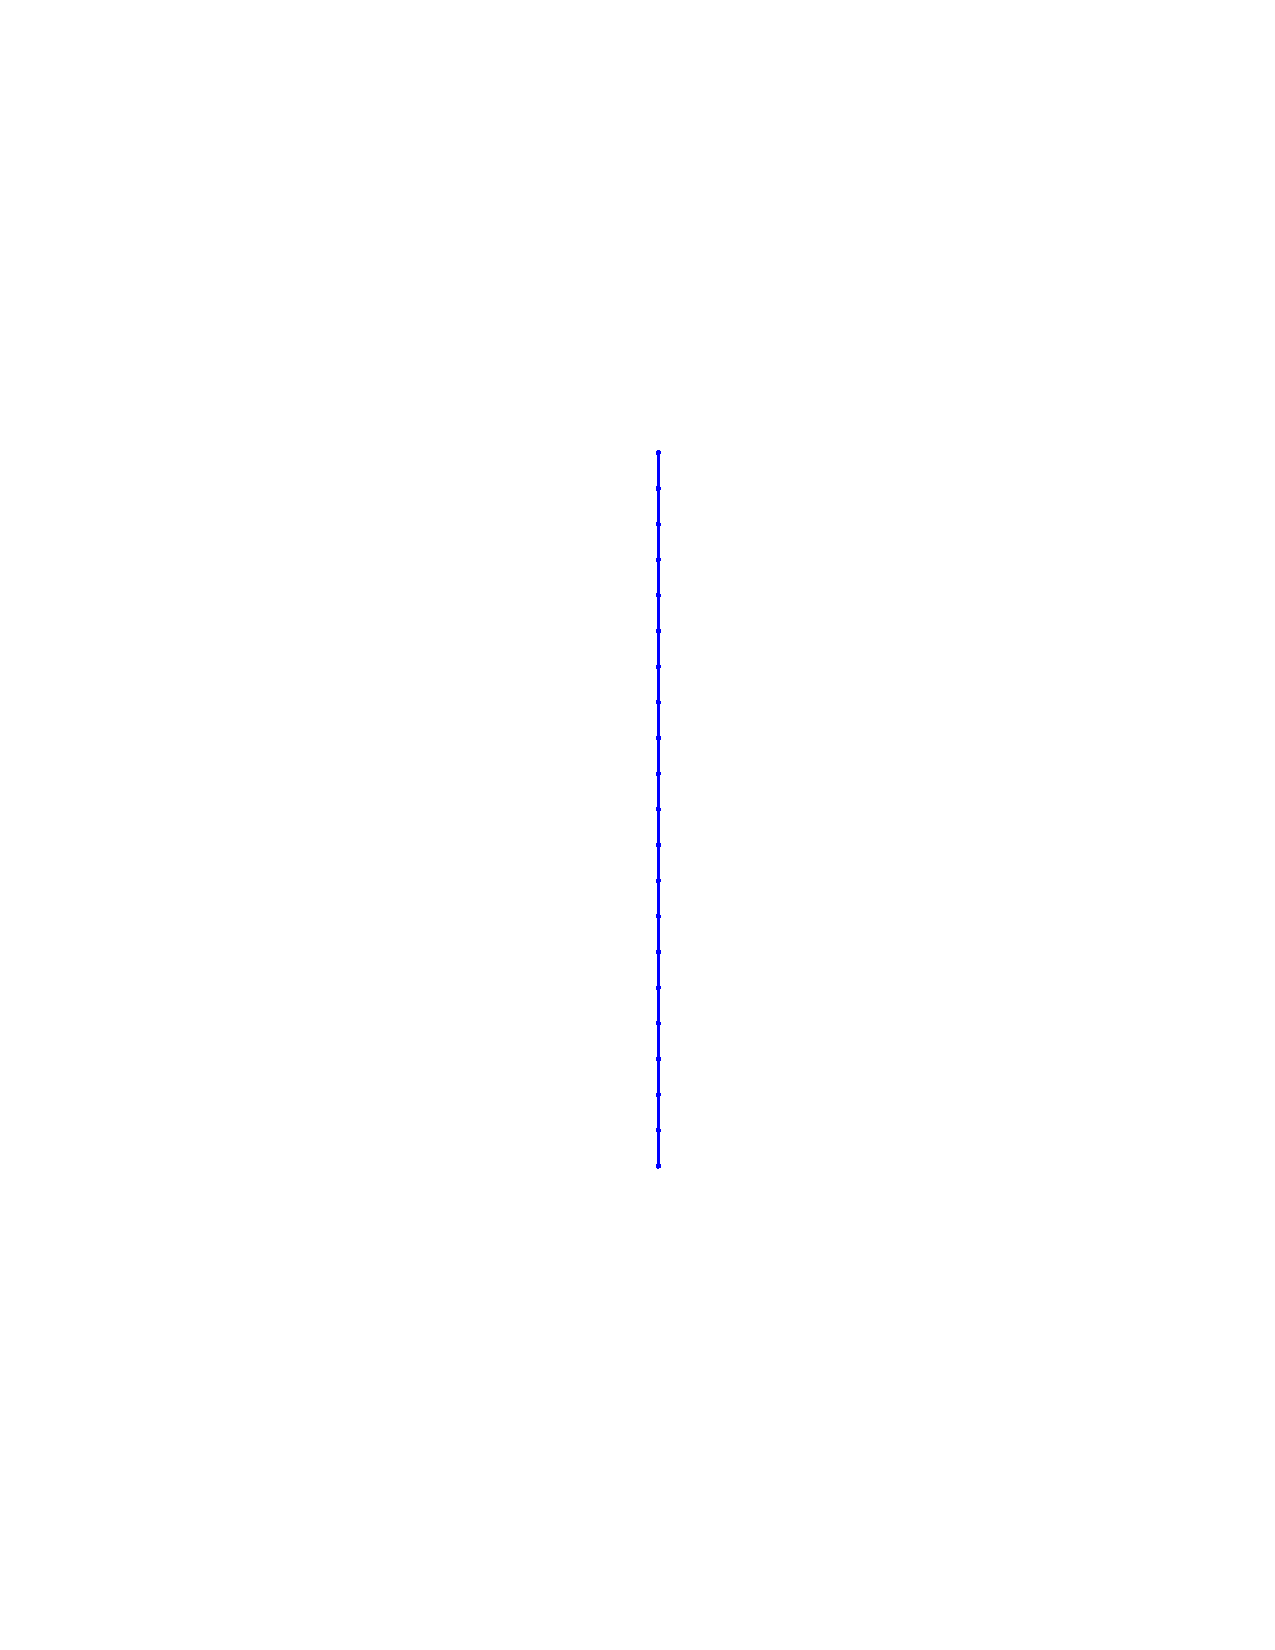
\includegraphics[trim={-5cm 5cm -5cm 5cm},
    width=.9\columnwidth,
    scale=2]
    {figures/method/trajectory-sampled}
    \caption{Trajectory sampled 21 times.}
  \end{minipage} \; %
  \begin{minipage}[r]{.45\columnwidth}
    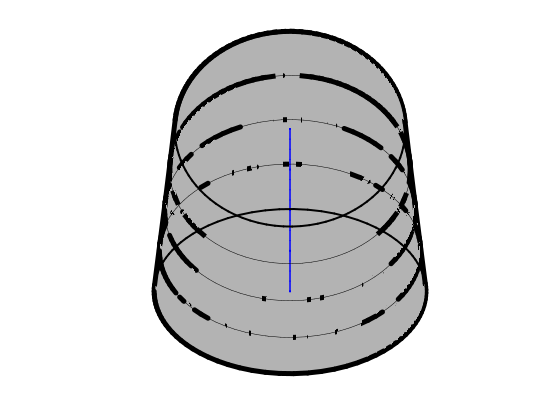
\includegraphics[trim={-5cm 5cm -5cm 5cm},
    width=.9\columnwidth,
    scale=2]{figures/method/funnel-sampled}
    \caption{The verified trajectory ellipsis overlaid at the sample times.}
    \label{fig:funnel-straight-sampled}
  \end{minipage}
\end{figure}


\subsection{Expanding the Size of the Funnels}

In general the funnels generated are computed only for the point model in
\cref{eq:dynamicalsystem}, and hence, in order to run the algorithm with a
model of some defined size, the funnels have to be expanded by the largest
radius of the model. Since the funnels are ellipsis around the point at the
trajectory that they verify, the funnels can be expanded by any radius with a
linear transformation. An expansion of a funnel around the point model used in
this paper can be seen in \cref{fig:expanded-funnel}.


\begin{figure}[!t]
  \centering 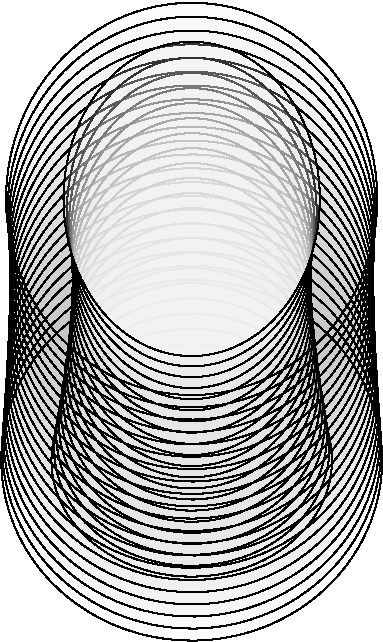
\includegraphics[scale=.3]{figures/method/expanded-funnel}
  \caption[The expanded experiment funnel]{The original funnel created from the point model, with a funnel
    expanded by a radius of 0.1 surrounding it.}
  \label{fig:expanded-funnel}
\end{figure}
